\documentclass[11pt]{article}

\usepackage{booktabs}
\usepackage{multirow}

\usepackage{amssymb}

\usepackage{fontspec}
% Libertine
\setmainfont[Ligatures={Common,TeX}]{Linux Libertine O}
\setsansfont{Linux Biolinum O}
\setmonofont{Inconsolata}

\usepackage{minted}
\newminted{julia}{}

\usepackage{geometry}
\geometry{
	xetex,
	textwidth=410pt
}

\hyphenpenalty 300

\newcommand{\cm}{$\checkmark$}

\title{Gaston \\[0.8cm] \large A plotting utility for Julia \\[0.8cm] v. 0.3}
\author{M. Bazdresch}
\date{\today}

\newcommand{\cmd}[1]{\texttt{#1}}

\begin{document}
\maketitle

\textbf{Please note:} Gaston is currently under development, and all functions
and definitions are subject to change from one version to the next, as we
figure out the best way to organize the code. Gaston has been tested on Linux
(Ubuntu 10.04 and Arch), with gnuplot 4.6 and WxWindows. It only supports the
wxt terminal.

\section{Introduction}

Gaston provides a way to plot scientific data using the Julia programming
language. It accomplishes this by harnessing gnuplot, a versatile and
time-tested plotting utility. Gaston also relies on gnuplot for interacting
with plots (zooming and rotating a plot with the mouse, for instance).

The primary purpose of Gaston is to provide easy-to-use functions to quickly
and conveniently plot the most common kinds of scientific and numeric data. It
is concerned with screen output only (although we plan to support printing to a
file in a future version), and supports the most common plot configurations
only. Tweaking a plot to produce a specific look or producing
publication-quality graphics are outside its scope.

\section{Installation}

To use Gaston, follow this procedure:

\begin{enumerate}

\item Save all files \cmd{gaston*.jl} somewhere convenient. Then,
	you may \cmd{cd} to that directory and start julia there, or do

\begin{juliacode}
push(LOAD_PATH, "/path/to/gaston/jl")
\end{juliacode}

Then, load the program with

\begin{juliacode}
load("gaston.jl")
\end{juliacode}

\item To run a demo, do

\begin{juliacode}
load("gaston_demo.jl")
demo()
\end{juliacode}

This will create a series of figures that illustrate the current capabilities
of the program. The same file may also serve as a guide on how to create
different types of plots.
\end{enumerate}

\section{Definitions}

A \textbf{figure} is an independent window, which contains a set of axes, on
which one or more \textbf{curves} are plotted. A figure may contain
\textbf{labels} (for instance, on each coordinate axis), a \textbf{title}, and a
\textbf{legend box} which identifies each curve. Gaston supports having any
number of figures open at the same time; however, gnuplot requires that only
one figure is able to offer mouse interactivity at a given time. Each figure is
identified by a unique \textbf{handle}. Handles are natural numbers.

A \textbf{curve} is defined by a set of coordinates. Two-dimensional curves
have \textbf{x} and \textbf{y} coordinates; in three dimensions, an additional
\textbf{z} coordinate must be specified. A curve also has several
\textbf{properties} that specify a plotting configuration (for instance, it may
have a \textbf{plotstyle}, a \textbf{linewidth}, a \textbf{linecolor}, etc),
which define how the curve is to be plotted.

\section{Plotting}

\subsection{Figures}

A figure may be created by the function \cmd{figure()}. Many plotting functions
create or reuse an existing figure, as needed (see each function's
documentation). Called with no arguments, \cmd{figure()} creates a new figure
with the smallest available handle. Called with an argument (which must be a
natural number), it will create a figure with that handle if no such figure
exists, or will select it (make it current) if it exists.

Selecting an existing figure may be useful, for instance, to make it mouse and
keyboard interactive.

Handles may be created in any numerical order.

This function always returns the handle of the current figure.

\subsection{Terminals}

Gaston supports plotting to the screen as well as printing the plots to files.
Two screen terminals are supported: \cmd{wxt} and \cmd{x11}. The \cmd{x11}
terminal is provided for use in systems that don't support WxWindows.

For printint to files, terminals \cmd{svg} and \cmd{gif} are supported. For
more details on printing, see section \ref{s:print} below.

To set the terminal type, use the command
\begin{juliacode}
set_terminal(term)
\end{juliacode}
where \cmd{term} is a string.

\subsection{2-D plotting}

There are two commands for two-dimensional plotting: \cmd{plot()} and
\cmd{histogram()}.

\subsubsection{plot()}

The \cmd{plot()} function takes any number of arguments, with the following
format:

\cmd{plot(\{h,\} \{x,\} y \{, property, value,...\} \{...\})}

\begin{itemize}
	\item If the optional argument \cmd{h} is provided, it is assumed to be the
		figure handle in which to plot.
		\begin{itemize}
			\item If the handle doesn't exist, a new figure is created.
			\item If it exists, the figure will be overwritten.
			\item If it is 0, then a new figure to plot in will be created,
				using the next handle available.
		\end{itemize}
		If it is not provided, then the current figure will be used and
		overwritten.
	\item The \cmd{x} and \cmd{y} arguments specifiy coordinates (they must be ranges, vectors, or
		two-dimensional arrays with a singleton dimension). If only \cmd{y} is
		provided, it is assumed to be the ordinate. If \cmd{x} and \cmd{y} are provided, they
		are assumed to be the abscissa and the ordinate, in that order.
	\item The coordinates may be followed by any number of
		\cmd{property}, \cmd{value} pairs. These are used to set the value of
		any of the curve's or the axes' properties (see section Reference,
		below). \cmd{property}s are always strings. The \cmd{value}s must be of
		the appropriate type.
	\item The pattern \cmd{\{x,\} y \{, property, value,...\}} may be repeated any
		number of times.
		\begin{itemize}
			\item Curve settings are always set for the immediately
				preceding curve.
			\item Axes settings may be specified at any time,
				and in the case of repeated properties, the last one set is the
				one that is used.
		\end{itemize}
	\item Properties may take the following values: \cmd{plotstyle},
		\cmd{legend}, \cmd{color},
		\cmd{marker}, \cmd{linewidth}, \cmd{pointsize}, \cmd{title},
		\cmd{xlabel}, \cmd{ylabel}, \cmd{box}, \cmd{axis}.
	\item Supported plotstyles are \cmd{lines}, \cmd{linespoints},
		\cmd{points}, \cmd{impulses} and \cmd{boxes}.
	\item plot() returns the handle of the figure that was plotted.
\end{itemize}

As an example, to plot an amplitude modulated signal and its envelope, we may
run the following code:

\begin{juliacode}
t = 0:0.0001:.15
carrier = cos(2pi*t*200)
modulator = 0.7+0.5*cos(2pi*t*15)
am = carrier.*modulator
plot(t,am,"color","blue","legend","AM DSB-SC","linewidth",1.5,
    t,modulator,"color","black","legend","Envelope",
    t,-modulator,"color","black","title","AM DSB-SC example",
    "xlabel","Time (s)","ylabel","Amplitude",
    "box","horizontal top left")
\end{juliacode}

\noindent which produces this plot:

\begin{center}
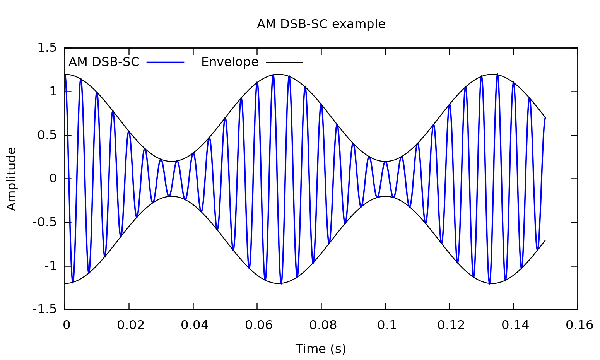
\includegraphics[width=10cm]{plotexample}
\end{center}

\subsubsection{histogram()}

The \cmd{histogram()} function plots a single histogram in a figure. It has the
following format:

\cmd{histogram(\{h,\} y \{, "bins", bins\} \{, "norm", norm\}
\{, property, value,...\})}

\begin{itemize}
	\item The optional argument \cmd{h} has the same meaning as in
		\cmd{plot()}.
	\item The histogram consists of boxes, where the height of each box is
		given by the number of elements of \cmd{y} that fall in a given range.
	\item \cmd{bins} specify the number of bins (boxes) that will be plotted.
	\item If \cmd{norm} is specified, the histogram will be normalized, so that
		the area under the histogram is equal to \cmd{norm}.
	\item The pairs \cmd{\{property, value,...\}} have the same meaning as in
		\cmd{plot()}.
	\item Properties may take the following values: \cmd{legend}, \cmd{color},
		\cmd{linewidth}, \cmd{title}, \cmd{xlabel}, \cmd{ylabel}, \cmd{box}.
	\item \cmd{histogram()} returns the handle of the figure that was plotted.
\end{itemize}

As an example, to plot an approximation of a Rayleigh density, we may run the
following code:

\begin{juliacode}
y = sqrt( randn(1000).^2 + randn(1000).^2 )
histogram(y,"bins",25,"norm",1,"color","blue","title","Rayleigh density (25 bins)")
\end{juliacode}

which produces this plot:

\begin{center}
	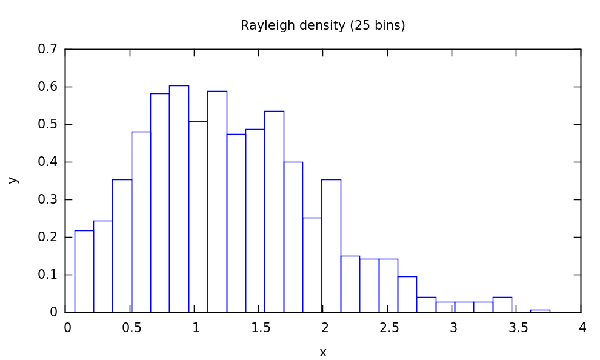
\includegraphics[width=10cm]{histexample}
\end{center}

\subsection{3-D plotting}

TBW

\subsection{Plotting images}

TBW

\section{Plotting with mid-level functions}

In addition to the plotting functions described in the section above, Gaston
offers a ``mid-level'' set of functions that allow plots to be created
step-by-step.

Having this mid-level layer has two benefits. One is that this layer is more
flexible and allows direct control over all aspects of the plot. For instance,
using high-level functions it is not currently possible to plot more than one
histogram, or a histogram and another curve, on the same figure. The mid-level
layer allows such combinations. Another example is an algorithm that builds
figures step-by-step as data becomes available, instead of waiting until all
the data needed has been produced.

A second benefit is that this layer abstracts Gaston's internal graphics
representation from the high-level layer. This means Gaston's whole back-end
may change without affecting the high-level functions; only the mid-level layer
would have to be adapted.

Also, much of Gaston's error checking and argument validation is performed at
this layer.

Please note that there is a single mid-level plot command, which is
\cmd{llplot()}. According to the type of coordinates and plotstyle, it will
figure out how to plot.

\subsection{2-D plotting}

Plotting proceeds in steps:
\begin{enumerate}
	\item Create or select a figure with \cmd{figure(i)}, where \cmd{i} is a
		positive integer.
	\item Add a curve (a set of coordinates plus a plot configuration), with
		\cmd{addcoords(x,y,conf)}. Here, \cmd{x} and \cmd{y} are vectors, and
		\cmd{conf} configures the plot and line styles, markers, legend, color,
		etc. Repeat this step for each curve you wish to include
		in the figure.
	\item Add a configuration for the entire figure (axis), with
		\cmd{addconf(conf)}, where \cmd{conf} contains the figure
		configuration.
	\item Issue the \cmd{llplot()} command.
\end{enumerate}

A curve configuration is created as follows:
\begin{enumerate}
	\item Create a default configuration with \cmd{c = CurveConf()}.
	\item \cmd{c} is a structure, each of whose fields controls one aspect of
		the curve's configuration. These fields may be set individually.
		Available fields are: \cmd{legend}, \cmd{plotstyle}, \cmd{color},
		\cmd{marker}, \cmd{linewidth}, and \cmd{pointsize}. For instance, to
		change a curve's color, do\footnote{Directly changing a structure's
		fields, instead of using setter functions, may be seen as non-idiomatic
		or inelegant. In this case we have decided to do the simplest thing
		that might possibly work.}

\begin{juliacode}
c.color = "blue"
\end{juliacode}

	See gnuplot's documentation to see the range of valid options.

\end{enumerate}

A figure (axis) configuration is created as follows:
\begin{enumerate}
	\item Create a default configuration with \cmd{a = AxesConf()}
	\item Just as in the case of a curve configuration, \cmd{a} is a structure
		whose fields may be modified. Available fields are: \cmd{title},
		\cmd{xlabel}, \cmd{ylabel}, \cmd{zlabel}, \cmd{box}, \cmd{axis}.
\end{enumerate}

Several rules apply:
\begin{itemize}
	\item You can create as many figures, each with as many curves, as desired.
	\item Generally, if you don't provide some of the data, it will be
		inferred. For example, calling \cmd{addcoords} with a single vector
		\cmd{y}
		will assume the \cmd{x} coordinate is \cmd{1:length(y)} and set up the
		default plot configuration.
	\item If you call \cmd{addcoords} with matrix arguments, each column will
		be interpreted as a different plot.
	\item Calling \cmd{addcoords()} will create a new figure if none have been
		created yet.
	\item Calling \cmd{llplot()} without an axis configuration will just use one
		by default.
	\item Gnuplot only provides mouse interaction support for the current
		figure. To use the mouse in a previously created figure \cmd{i}, just
		issue command \cmd{figure(i)}. This will also bring the figure to the
		front.
\end{itemize}

\subsubsection{2-D plotting styles}

Besides simply plotting a set of \cmd{x} and \cmd{y} coordinates, Gaston
supports other kinds of plots.

\textbf{Error bars and lines.} To add error bars or lines, just call
\cmd{addcoords()} with one or two extra coordinates, and configure the
plotstyle accordingly.

\textbf{Histograms.} To plot the histogram of a data vector \cmd{data} with
\cmd{b} bins, first use the auxiliary function \cmd{(x,y) = histdata(data,b)}
to create \cmd{x} and \cmd{y} coordinates that may be plotted with the
\cmd{boxes} plotstyle.

\subsection{3-D plotting}

The same rules apply, except that \cmd{addcoords()} should be called as
\cmd{addcoords(x,y,Z)}, where \cmd{Z} is a matrix whose element \cmd{j,k}
corresponds to some function of \cmd{x[j],y[k]}.

For convenience, a function \cmd{Z = meshgrid(x,y,f)} is provided. Called with
\cmd{x}, \cmd{y} coordinates and a function \cmd{f}, it will return a matrix
that may be used to plot \cmd{f}.

\subsection{Image plotting}

Two image plotstyles are supported: \cmd{image} and \cmd{rbgimage}. At the
moment Gaston requires that a figure contains only one image (and no other
curves). This restriction will be removed in future versions.

\textbf{Scalar image.} To plot a matrix \cmd{Z} as a figure, use
\cmd{addcoords([],[],Z)} with empty \cmd{x}, \cmd{y} coordinates and \cmd{Z} as
third argument, and set the plotstyle to \cmd{image}. Element \cmd{(j,k)} of
\cmd{Z} corresponds to element \cmd{(j,k)} in the plot, and its value determines
the color at that point.

\textbf{RGB image.} To plot an RGB image, the matrix \cmd{Z} must be three
dimensional. The first and second dimensions correspond to the value at each
point in the image.  The third dimension specifies red, green and blue values
at each point.  Finally, set the plotstyle to \cmd{rgbimage}.

\subsection{Printing to a file}
\label{s:print}

Gaston supports plotting a figure to a file instead of the screen
(\textit{printing} a file). Currently
supported are SVG and GIF files. There are two ways to print figures.

\subsubsection{Printing a single figure}

If you have a figure on screen that you want to print, you have to change the
terminal type, specify the filename, and then select the figure. For example,
if you want to print the figure with handle 10 to a GIF file named
\cmd{test.gif}, you would issue these commands:
\begin{juliacode}
set_terminal("gif")
set_filename("test.gif")
figure(10)
set_terminal("wxt")
\end{juliacode}
The final \cmd{set\_terminal} will allow subsequent plot commands to go to the
screen again.

\subsubsection{Always print to files}

If you want regular plot commands to print to files instead of showing the
plots on the screen, just set the terminal type and filename at the start of
your session. For example, Gaston may beused in a webserver that reads SVG
plots from a pipe; this may be set up as follows:
\begin{juliacode}
set_terminal("svg")
set_filename("|serverpipe")
plot(sin(-3:0.01:3),"title","SVG test")
\end{juliacode}
The plot command in the last line will cause the SVG data representing the
figure to be sent to the pipe \cmd{serverpipe}.

\section{Reference}

Note: In this section, at least superficial knowledge of Julia and gnuplot is
assumed. Please refer to the respective documentation for more details.

\subsection{Curve configuration}

A given curve's configuration is stored in a structure of type \cmd{CurveConf}.
This structure has the following fields:

{\small
\begin{center}
\begin{tabular}{lll}
	\toprule
	\textbf{Field} & \multicolumn{1}{c}{\textbf{Notes}} &
	\multicolumn{1}{c}{\textbf{Meaning in gnuplot}} \\
	\midrule
	\cmd{legend} & The text that appears in the legend box. & Argument of
	\cmd{title}. \\
	\cmd{plotstyle} & How the curve will be plotted. & Argument of \cmd{with}.
	\\
	\cmd{color} & The curve color. & Argument of \cmd{linecolor rgb}. \\
	\cmd{marker} & The marker name. & Argument of \cmd{pointtype}. \\
	\cmd{linewidth} & The curve line width; must be a positive number. &
	Argument of \cmd{linewidth}. \\
	\cmd{pointsize} & The marker size; must be a positive number. & Argument
	of \cmd{pointsize}. \\
	\bottomrule
\end{tabular}
\end{center}}

The types, default and valid values for each field are given in the following
table.

{\small
\begin{center}
	\begin{tabular}{lp{1.5cm}p{2cm}p{7.5cm}}
	\toprule
	\textbf{Field} & \textbf{Type} & \textbf{Default value} & \textbf{Valid values} \\
	\midrule
	\cmd{legend} & \cmd{String} & \cmd{""} & Any string. \\
	\cmd{plotstyle} & \cmd{String} & \cmd{lines} & \cmd{lines}, \cmd{linespoints},
	\cmd{points}, \cmd{impulses}, \cmd{errorbars}, \cmd{errorlines},
	\cmd{pm3d}, \cmd{boxes}, \cmd{image}, \cmd{rgbimage}. \\
	\cmd{color} & \cmd{String} & \cmd{""} & \cmd{""}, any gnuplot color name,
	or a color specified in a string in the format \cmd{"\#RRGGBB"}. \\
	\cmd{marker} & \cmd{String} & \cmd{""} & \cmd{""}, \cmd{+}, \cmd{x}, \cmd{*}, \cmd{esquare},
	\cmd{fsquare}, \cmd{ecircle}, \cmd{fcircle}, \cmd{etrianup},
	\cmd{ftrianup}, \cmd{etriandn}, \cmd{ftriandn}, \cmd{edmd}, \cmd{fdmd} (run
	\cmd{test} in gnuplot terminal). \\
	\cmd{linewidth} & \cmd{Real} & 1 & Any real number \\
	\cmd{pointsize} & \cmd{Real} & 0.5 & Any real number \\
	\bottomrule
\end{tabular}
\end{center}}

Notes: When \cmd{color} or \cmd{marker} are set to the empty string, gnuplot will use
its own default values. Gaston does not verify that the color name provided is
valid. You can see a list of valid colornames running \cmd{show colornames} in
a gnuplot terminal.

The following table lists the marker names and corresponding symbols.

{\small
\begin{center}
\begin{tabular}{lc}
	\toprule
	\textbf{Marker name} & \textbf{Symbol} \\
	\midrule
	\cmd{+} & + \\
	\cmd{x} & $\times$ \\
	\cmd{*} & $\ast$ \\
	\cmd{esquare} & $\square$ \\
	\cmd{fsquare} & $\blacksquare$ \\
	\cmd{ecircle} & $\circ$ \\
	\cmd{fcircle} & ● \\
	\cmd{etrianup} & △ \\
	\cmd{ftrianup} & ▲ \\
	\cmd{etriandn} & ▽ \\
	\cmd{ftriandn} & ▼ \\
	\cmd{edmd} & ◇ \\
	\cmd{fdmd} & ◆ \\
	\bottomrule
\end{tabular}
\end{center}}

\subsection{Axes configuration}

There may be only one configuration per figure. This configuration is stored in
a structure of type \cmd{AxesConf}, which has the following fields:

{\small
\begin{center}
\begin{tabular}{lll}
	\toprule
	\textbf{Field} & \multicolumn{1}{c}{\textbf{Notes}} &
	\multicolumn{1}{c}{\textbf{Meaning in gnuplot}} \\
	\midrule
	\cmd{title} & The figure's title & \cmd{title-spec} \\
	\cmd{xlabel} & Abscissa's label & Argument to \cmd{set xlabel} \\
	\cmd{ylabel} & Ordinate's label & Argument to \cmd{set ylabel} \\
	\cmd{zlabel} & Z-axis label & Argument to \cmd{set zlabel} \\
	\cmd{box} & Legend box configuration & Argument to \cmd{set key} \\
	\cmd{axis} & Axis scale & Argument to \cmd{set logscale} \\
	\bottomrule
\end{tabular}
\end{center}}

The types, default and valid values for each field are given in the following
table.

{\small
\begin{center}
	\begin{tabular}{lp{1.5cm}p{2cm}p{7.5cm}}
	\toprule
	\textbf{Field} & \textbf{Type} & \textbf{Default value} & \textbf{Valid values} \\
	\midrule
	\cmd{title} & \cmd{String} & \cmd{"Untitled"} & Any string \\
	\cmd{xlabel} & \cmd{String} & \cmd{"x"} & Any string \\
	\cmd{ylabel} & \cmd{String} & \cmd{"y"} & Any string \\
	\cmd{zlabel} & \cmd{String} & \cmd{"z"} & Any string \\
	\cmd{box} & \cmd{String} & \cmd{"inside vertical right top"} & Any valid
	string \\
	\cmd{axis} & \cmd{String} & \cmd{""} & \cmd{""}, \cmd{normal},
	\cmd{semilogx}, \cmd{semilogy}, \cmd{loglog}  \\
	\bottomrule
\end{tabular}
\end{center}}

Notes: Gaston does not verify that \cmd{box} contains a valid \cmd{set key}
argument. The \cmd{axis} values follow Matlab's conventions for logscale axes;
Gaston translates them to gnuplot's equivalents.

\subsection{Changing default configuration}

Gaston provides functions to change the default values listed above. There is
one function per each property, both for curves and for axes. For example, a
Spanish speaker may wish to change the default value for figure titles from
``Untitled'' to ``Sin título''. This is achieved by
\begin{juliacode}
set_default_title("Sin título")
\end{juliacode}
and, from that point on, any figure with an unspecified title will be titled
thus.

Functions to change the defaults have the form \cmd{set\_default\_*(arg)},
where \texttt{*} is the property name and \cmd{arg} is the new default
value (must be of the appropriate type).

\subsection{Plot types}

In this section, we describe how Gaston decides which kind of plot to produce
(2-d, 3-d, or image), based on the available coordinates and specified plot
style.

In the following table, a checkmark (\cm) means that the coordinate has been
specified by the user in either a mid-level or high-level command (\cmd{y}
coordinates, if not specified, are calculated by Gaston, and are not included
in the following table. The same applies to \cmd{yhigh}).

{\small
\begin{center}
	\begin{tabular}{lcccl}
	\toprule
	\textbf{plotstyle} & \textbf{x} & \textbf{Z} & \textbf{ylow} &
	\textbf{Gnuplot command} \\
	\midrule
	\multirow{2}{*}{\cmd{lines}}
	& \cm &     &  & \cmd{plot with lines} \\
	& \cm & \cm &  & \cmd{splot with lines} \\
	\cmidrule(r){2-5}
	\multirow{2}{*}{\cmd{linespoints}}
	& \cm &     &  & \cmd{plot with linespoints} \\
	& \cm & \cm &  & \cmd{splot with linespoints} \\
	\cmidrule(r){2-5}
	\multirow{2}{*}{\cmd{points}}
	& \cm &     &  & \cmd{plot with points} \\
	& \cm & \cm &  & \cmd{splot with points} \\
	\cmidrule(r){2-5}
	\multirow{2}{*}{\cmd{impulses}}
	& \cm &     &  & \cmd{plot with impulses} \\
	& \cm & \cm &  & \cmd{splot with impulses} \\
	\cmidrule(r){2-5}
	\cmd{boxes}       & \cm &  &     & \cmd{plot with boxes} \\
	\cmd{errorbars}   & \cm &  & \cm & \cmd{plot with errorbars} \\
	\cmd{errorlines}  & \cm &  & \cm & \cmd{plot with errorlines} \\
	\cmidrule(r){2-5}
	\multirow{2}{*}{\cmd{pm3d}}
	&     & \cm &  & \cmd{splot with pm3d} \\
	& \cm & \cm &  & \cmd{splot with pm3d} \\
	\cmidrule(r){2-5}
	\cmd{image}       &  & \cm &  & \cmd{plot with image} \\
	\cmd{rgbimage}    &  & \cm &  & \cmd{plot with rgbimage} \\
	\bottomrule
\end{tabular}
\end{center}}

Any other combination of coordinates and plotstyle produces undefined behavior
-- we try to identify invalid combinations and produce an error, but this is
not guaranteed. Please note that mixing 2-d and 3-d plots on the same figure
also produces undefined behavior.

\subsection{Global variables}

TBW

\subsection{Types}

TBW


\end{document}
